%\documentclass{article}
\documentclass[a4paper,10pt]{article}
\usepackage[utf8]{inputenc}
\usepackage{graphicx}
\usepackage{url}
\usepackage{float}
\usepackage{times}
\usepackage{multirow}
\usepackage{listings}
\usepackage{times}
\usepackage{paralist}
\usepackage{epsfig}
\usepackage{subfigure}
\usepackage[hypertex]{hyperref}
\usepackage{subfigure}
\usepackage{color}

\textwidth = 6.0in
\textheight = 9.0in
\oddsidemargin = 0.5in
\evensidemargin = 0.0 in
\topmargin = 0.0 in
\headheight = 0.0 in
\headsep = 0.0 in


\usepackage{ifpdf}

\newcommand{\I}[1]{\textit{#1}}
\newcommand{\B}[1]{\textbf{#1}}
\newcommand{\BI}[1]{\textbf{\textit{#1}}}
\newcommand{\T}[1]{\texttt{#1}}

\setlength\topmargin{0in}
\setlength\headheight{0in}
\setlength\headsep{0in}
\setlength\textheight{9in}
\setlength\textwidth{6.5in}
\setlength\oddsidemargin{0in}
\setlength\evensidemargin{0in}
\setlength\parindent{0.1in}
\setlength\parskip{0.25em}


\ifpdf
 \DeclareGraphicsExtensions{.pdf, .jpg}
\else
 \DeclareGraphicsExtensions{.eps, .ps}
\fi

\newcommand{\jha}[1]{ {\textcolor{red} { ***Jha: #1 }}}

\begin{document}

\title{\large Characterising and Developing Adaptive Scientific
  Applications with Hard to Predict Runtime Resource Requirements}

\author{Shantenu Jha$^{1,2,3}$, Yaakoub El-Khamra$^{1}$, Hartmut Kaiser$^{1}$, \\ Andre Merzky$^{1}$, Ole Weidner$^{1}$ \\
  \small{\emph{$^{1}$Center for Computation \& Technology, Louisiana State University, USA}}\\
  \small{\emph{$^{2}$Department of Computer Science, Louisiana State
      University, USA}}\\
  \small{\emph{$^{3}$e-Science Institute, University of Edinburgh,
      UK}}}

\maketitle

There are large number of applications that have irregular execution
characteristics and highly variable resource requirements which are
very difficult to predict in advance.  The irregularity may manifest
itself in either the total time required to run, time for run for each
sub-task, the number of sub-tasks, or irregular communication between
the sub-tasks , to name just a few.  From the run-time environment
perspective, computational Grids are almost by definition,
characterised as dynamic and heterogeneous environments.  They are
dynamic due to time-dependent resource loads, availability and access
patterns; the aggregation of specialised resources in different
administrative domains is one source of the heterogeneity.  We believe
that novel, distributed applications must be dynamic and have support
for adaptivity -- due to either changes in external factors (eg
resource availabilty) or due to internal factors (eg more sub-tasks
need to be computed).  It is important to note, that traditional,
monolithic HPC programs are typically not adaptive in response to
changing conditions due to either scenario.

In principle there is a difference between ``hard to predict'' and
irregular execution on the one hand and adaptivity on the other.
Application-level adaptivity however, is a powerful and simple way to
respond to changing resource requirements or availability.  But there
are many challenges to application level adaptivity -- not least of
which are a lack of advanced programming models for developing
adaptive application, insufficient run-time support for the adaptive
aspects and the complexity associated with application-level
scheduling.

%to both externally and internally triggered changes.
%Thus applications need to be able to adapt to 

% Most applications and run-time systems for distributed applications
% assume that the application and any sub-tasks during the course of an
% application's life-time, will display a well-defined, static execution
% characteristics.  This makes it hard to use regular, production level
% infrastructure for such applications.

We have developed and investigate two distinct adaptive applications;
both are capable of responding to changing resource availability and
performance.  In Ref~\cite{saga_escience07x}, we developed an
network-intensive application that was able to determine the best
run-time configuration based upon bandwidth requirements and network
performance. In Ref~\cite{saga_tg08}, we showed how an application
could use computational sensors to determine the best set of resources
to launch a varying set of sub-tasks onto.  In the latter case, there
were additional constraints of global synchronisation and the need to
lower the time to completion.

As a consequence of the resource requirements being dynamic and
unpredictable, coupled with dependence on the execution trajectory and
resources used, it is difficult to define a scheduling strategy that
will be effective throughout the complete execution of an
applications; hence static resource mapping is generally not an
option.  It can be argued that the logic for adapting to resource
requirement changes from within the application are best addressed at
the application level. The constraints and design-space for
application-level adaptivity however, are not well understood.  In
general, such applications are hard to develop and deploy; but in
spite of their importance, they have surprisingly received little
support for the development and deployment.  Also as pointed out in
Ref~\cite{apples03} it is not easy to programmatically adapt the
application performance characteristics so as to be usable by a wide
range of application classes.

In this paper, we discuss our approach to the design and development
of three adaptive applications -- early prototypes that continue to
undergo refinement.  A common feature in our approach is the use of
the the Simple API for Grid Applications (SAGA)~\cite{saga_gfd90}.
%, which attempts to
%consolidate community effort and make ends meet by employing a
%top-down approach to distributed computing software infrastructure.
SAGA is the first comprehensive attempt to provide a programmatic
approach for the development of applications so as to utilize
distributed environments -- either by design or by virtue of
deployment.  In addition to simplifying the programming environment
for application developers, SAGA insulates applications from
technological version changes and other implementation specific
details that regularly occur in the lower layers of the software
stack.

Collectively, the applications we investigate span a broad range of
the spectrum of {\it irregular characteristics} that applications
have.  In addition to the three applications we develop, there exist
several other well known examples of applications with irregular
run-time characteristics eg., GridSAT~\cite{gridsat03,
  majority_voting}. We will use these applications as the basis for
defining the core characteristics (vectors) of applications with
irregular run-time characteristics and will help define the design
space of when adaptivity should be embedded at the application level
(eg using SAGA coupled with another framework such as Cactus) versus
when it should be handled using system-level frameworks (eg Charm++)
or another level altogether.

% that have been able to respond to changes in, or optimise
% deployment configuration based upon network characteristics and/or
% based upon batch-queue characateristics (using the batch-queue
% predictor).  Our results are reported in references
% ~\cite{saga_escience07x, saga_tg08}.

% Not only is the development of
% such applications difficult, but the effective deployment of such
% application remains a challenge.

% For these applications the resource requirement is dynamic and
% unpredictable; interestingly, the resource requirements and
% utilization might possibly be dependent upon both the execution
% trajectory and underlying infrastructure.  

% Interestingly the variable execution pattern and resource requirement
% is accompanied by, though not causally related to, a horizontal
% coupling between the distributed jobs, say for example, a randomly
% occuring global (or even local) exchange points or global
% synchronization points.

% we adopt in this paper attempts to be the first to provide a
% programmatic ability for a general class of applications from a wide
% range of distributed patterns.

\begin{figure}
\begin{center}
  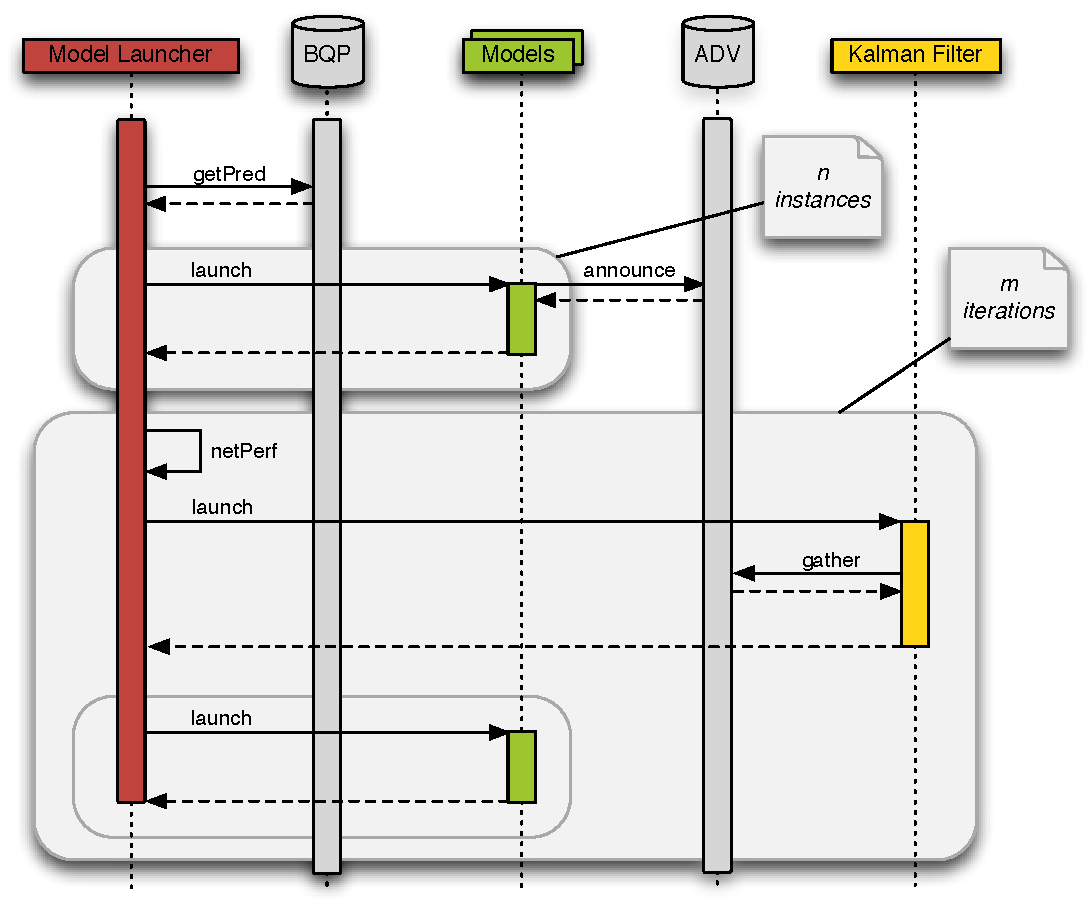
\includegraphics[scale=0.4]{SequenceDiagram}
\end{center}
\caption{A schematic illustration of control flow of an irregular,
  hard to predict application, taken from Ref~\cite{saga_tg08}.  The
  application is a SAGA-Cactus based ensemble Kalman filter
  application, where models are generated and these are mapped to
  appropriate resources. This is done based upon the number of grid
  points in the model (which in turn determines the number of
  processors and memory) and the projected run-time (which is based
  upon estimated number of iterations).  An optimal resource --
  defined as that resource with the highest chances of finishing a job
  with the prescribed characteristics (number of processors, duration)
  first is chosen to launch the sub-tasks.  After all models (n
  instances) in a given stage have finished there is a global
  synchronization point which in turn is the basis for providing
  models for the next stage (m iterations). It is difficult to
  determine the values of {\bf n} and {\bf m} {\it a priori}}
\label{fig:controlflow}
\end{figure}

%   Specifically high-level overview of the control flow for the
%  To a first approximation data from BQP is utilized
%   Obviously this is just a best effort guesstimate, as the actual
%   run-time (number of iterations) is difficult to get correct (as it
%   depends upon convergence to a value). 

% HPC Grids such as the TeraGrid and DEISA have definitely provided a
% massive increase in the computing power available for scientific
% applications, but this is due to the individual parts, and has nothing
% to do with the sum of the parts, i.e., the increase is not nearly
% enough because applications are able to use distributed resources in a
% coupled or coordinated manner.  The future of the
% TeraGrid~\cite{teragridfuture} is at best uncertain; this is in part
% due to the fact that the TeraGrid has had limited success in
% engendering novel applications or usage modes.  The problem is however
% not localised to the TeraGrid; there exists a general inability to
% provide the platform for any new distributed programming paradigm or
% novel application class.  For example, it remains difficult to harness
% more than one resource at other high-end distributed infrastructure,
% such as DEISA for the purposes of a single application.

\bibliographystyle{IEEEtran} 
\bibliography{saga,saga_tg08}

\end{document}

% that exhibit such characteristics: Replica Exchange Simulations
% parallel ensemble Kalman filter (PEnKF)
% two newly developed applications -- 

%which has varying resource requirements and execution characteristics. 

%    Even for relatively small input problem sizes at each stage, up to
%    several hundred models are generated which require from one to
%    sixteen processors to solve efficiently; however, the distribution
%    of the number of jobs and the run time-to-completion for a given
%    processor count varies by up to an order of magnitude.  As a
%    consequence of irregular execution characteristics and dynamic
%    resource requirements, it is difficult to predict effective
%    resource mapping {\it a priori} and to use static scheduling
%    techniques.  We demonstrate how the use of appropriate programming
%    abstractions like SAGA and Cactus enable run-time resource
%    selection based upon the application specific characteristics and
%    the effective development of applications with non-trivial
%    requirements.  As proof of concept we deploy our application on the
%    TeraGrid and show the effective and coupled utilization of several
%    heterogeneous resources.

%    A key impediment to accelerated development of Grid applications
%    and consequently the uptake of Grids is the scarcity of high-level
%    application programming abstractions that bridge the gap between
%    existing Grid middle-ware and application-level needs.

% Application developers are daunted by the complexity of the vast array
% of low-level Grid and distributed computing software APIs that
% currently exist; APIs have traditionally been developed using a
% bottom-up approach that exposes the broadest possible functionality.
% Coding using these bottom-up APIs requires extremely verbose code to
% implement even the simplest of application-level capabilities.  Many
% Grid computing projects~\cite{gat, cog, realitygrid} recognized the
% need for higher-level programming abstractions to simplify the use of
% distributed computing for application developers.



% There exist a large class of applications for which the individual job
% run time characteristics are inherently difficult to predict and plan
% for.  In addition to Kalman filters~\cite{DataAssim, KalmanPaper},
% there are a class of ``first principles'' Grid applications such as
% GridSAT~\cite{gridsat03} and applications which are based upon
% resource aware ``learning'' algorithms~\cite{ majority_voting}, for
% which it is both difficult to estimate precisely the resource
% requirements while explicitly needing to marshal the distributed
% resources. 

% There exist several well known examples of distributed applications
% which in turn have multiple pleasingly distributable jobs (or
% sub-applications), that are either typically uncoupled or the coupling
% is between the master and client application.

% however, providing application level adaptivity is a fundamental way
% to address these characterisitcs.
